\section{Relation $\gamma$ between the perimeter and the root square value of area}

In this section we analyze the relation $\gamma$, between the perimeter $P$ 
and the root square value of area $A$, so that
\begin{equation}
\gamma=\frac{P}{\sqrt{A}}.
\end{equation}
They will be calculated the $\gamma$ value of a triangle, a rectangle, and a circle. 

%%%%%%%%%%%%%%%%%%%%%%%%%%%%%%%%%%%%%%%%%%%%%%%%%%%%%%%%%%%%%%%%%%%%%%%%%%%%%%%%
\begin{comment}
\subsection{$\gamma$ value of a circle or $\gamma_c$}
The perimeter of a circle of radius $r$  is equal to $P_c=2 \pi r$, 
and the area $A_c=\pi r^2$. Thus, the value
\begin{equation}
\gamma_c=\frac{P_c}{\sqrt{A_c}}=2\sqrt{\pi}\approx 3.5449.
\end{equation}
\end{comment}

%%%%%%%%%%%%%%%%%%%%%%%%%%%%%%%%%%%%%%%%%%%%%%%%%%%%%%%%%%%%%%%%%%%%%%%%%%%%%%%%
\subsection{$\gamma$ value of an ellipse or $\gamma_e$}
\label{subsec:gammae}
The perimeter of an ellipse, with width $2a$ and height $2b$; 
it is equal to $P_e=4\int_{0}^{\frac{\pi}{2}}{\sqrt{a^2-(a^2-b^2)sin^2(\theta)}d\theta}$; 
 with an area $A_e=\pi ab$ \cite[pp. 702]{larson2010calculus}. Thus, the value
\begin{equation}
\gamma_e(a,b)=\frac{P_e}{\sqrt{A_e}}=\frac{4\int \limits_{0}^{\frac{\pi}{2}}{\sqrt{a^2-(a^2-b^2)sin^2(\theta)}d\theta}}{\sqrt{\pi ab}}.
\end{equation}
The $\gamma_e(a,b)$ function generates a surface as showed in the Fig. \ref{fig:section1-gammae}.
\begin{figure}[h!]
\centering
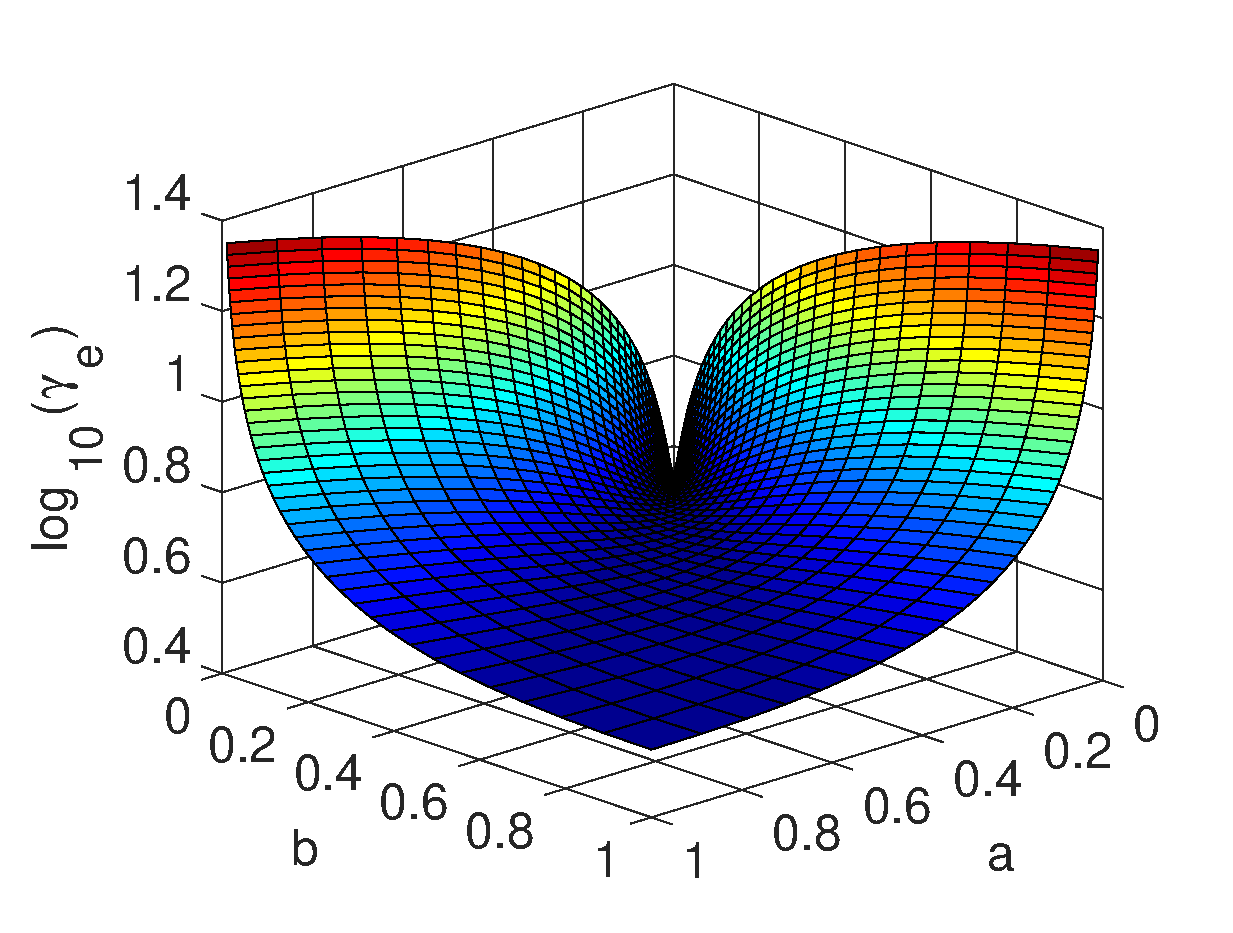
\includegraphics[width=0.45\textwidth]{section1-gammae.eps}
\caption{Surface generated by some possible values of $log_{10}(\gamma_e(a,b))$.}
\label{fig:section1-gammae}
\end{figure}
To obtain the minimum value of this surface we calculate $\frac{\partial \gamma_e(a,b)}{\partial a}=0$
and $\frac{\partial \gamma_e(a,b)}{\partial b}=0$, so that
\begin{equation}
\frac{\partial \gamma_e(a,b)}{\partial a}=
\frac{1}{\sqrt{\pi ab}}\left( \frac{\partial P_e(a,b)}{\partial a}-\frac{P_e(a,b)}{2 a} \right)=0,
\end{equation}
\begin{equation}
\frac{\partial \gamma_e(a,b)}{\partial b}=
\frac{1}{\sqrt{\pi ab}}\left( \frac{\partial P_e(a,b)}{\partial b}-\frac{P_e(a,b)}{2 b} \right)=0.
\end{equation}
Of this equation we deduce that the minimum value is $\gamma_e(a,b)$ is reach when
\begin{equation}
P_e(a,b)=k_a\sqrt{b}=k_b\sqrt{a}=k\sqrt{a b}.
\end{equation}
This can be obtained if $a=b$, where $P_e(a,a)=2\pi \sqrt{a^2}$
and $\gamma_e(a,a)=2 \sqrt{\pi} \approx 3.5449$; so that
\begin{equation}
2 \sqrt{\pi} \leq \gamma_e.
\end{equation}
%%%%%%%%%%%%%%%%%%%%%%%%%%%%%%%%%%%%%%%%%%%%%%%%%%%%%%%%%%%%%%%%%%%%%%%%%%%%%%%%
\subsection{$\gamma$ value of a rectangle or $\gamma_r$}
\label{subsec:gammar}
The perimeter of a rectangle, of sides with lengths  $a$ and $b$; 
it is equal to $P_r=2 (a+b)$; 
 with an area $A_r=ab$. Thus, the value
\begin{equation}
\gamma_r(a,b)=\frac{P_r}{\sqrt{A_r}}=\frac{2(a+b)}{\sqrt{ab}}.
\end{equation}
The $\gamma_r(a,b)$ function generates a surface as showed in the Fig. \ref{fig:section1-gammar}.
\begin{figure}[h!]
\centering
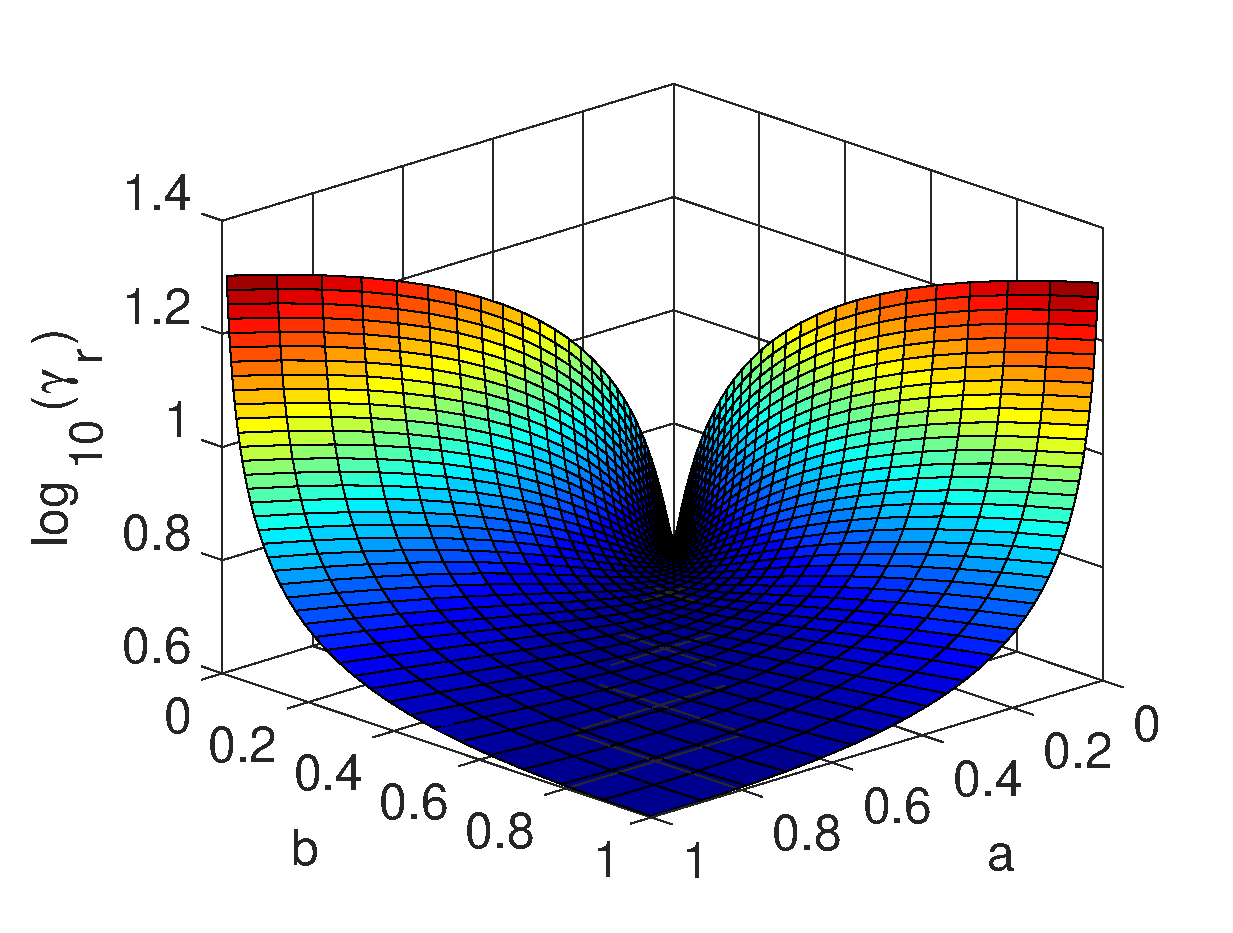
\includegraphics[width=0.45\textwidth]{section1-gammar.eps}
\caption{Surface generated by some possible values of $log_{10}(\gamma_r(a,b))$.}
\label{fig:section1-gammar}
\end{figure}
To obtain the minimum value of this surface we calculate $\frac{\partial \gamma_r(a,b)}{\partial a}=0$
and $\frac{\partial \gamma_r(a,b)}{\partial b}=0$, so that
\begin{equation}
\frac{\partial \gamma_r(a,b)}{\partial a}=\frac{2}{\sqrt{ab}}-\frac{a+b}{a\sqrt{ab}}=0,
\end{equation}
\begin{equation}
\frac{\partial \gamma_r(a,b)}{\partial b}=\frac{2}{\sqrt{ab}}-\frac{a+b}{b\sqrt{ab}}=0.
\end{equation}
Of this equation we deduce that the minimum value is $\gamma_r(a,b)$ is reach when $a=b$;
this mean when $\gamma_r(a,a)=4$; so that
\begin{equation}
4 \leq \gamma_r.
\end{equation}

%%%%%%%%%%%%%%%%%%%%%%%%%%%%%%%%%%%%%%%%%%%%%%%%%%%%%%%%%%%%%%%%%%%%%%%%%%%%%%%%
\subsection{$\gamma$ value of a triangle or $\gamma_t$}

The perimeter of a triangle, of sides with lengths  $a$, $b$ and $c$; 
it is equal to $P_t=a+b+c$; 
 with an area\footnote{Calculated using the Heron theorem.} $A_t=\sqrt{s(s-a)(s-b)(s-c)}$,
where $s=(a+b+c)/2$ \cite[pp. 253]{sterling2013algebra}. 
Thus, we can calculate the value
\begin{equation}
\gamma_t(a,b,c)=\frac{P_t}{\sqrt{A_t}}=\frac{a+b+c}{\sqrt[4]{s(s-a)(s-b)(s-c)}}.
\end{equation}

The $\gamma_t(a,b,c)$ function generates a solid with different values $\gamma_t$ to each point $\{a,b,c\}$
that can describe a trinagle, with this purpose we use the  triangle 
inequality\footnote{$a < b+c$, $b < a+c$ and $c < a+b$} \cite[pp. 17]{ross1980elementary};
the Fig. \ref{fig:section1-gammat} show this result.
\begin{figure}[h!]
\centering
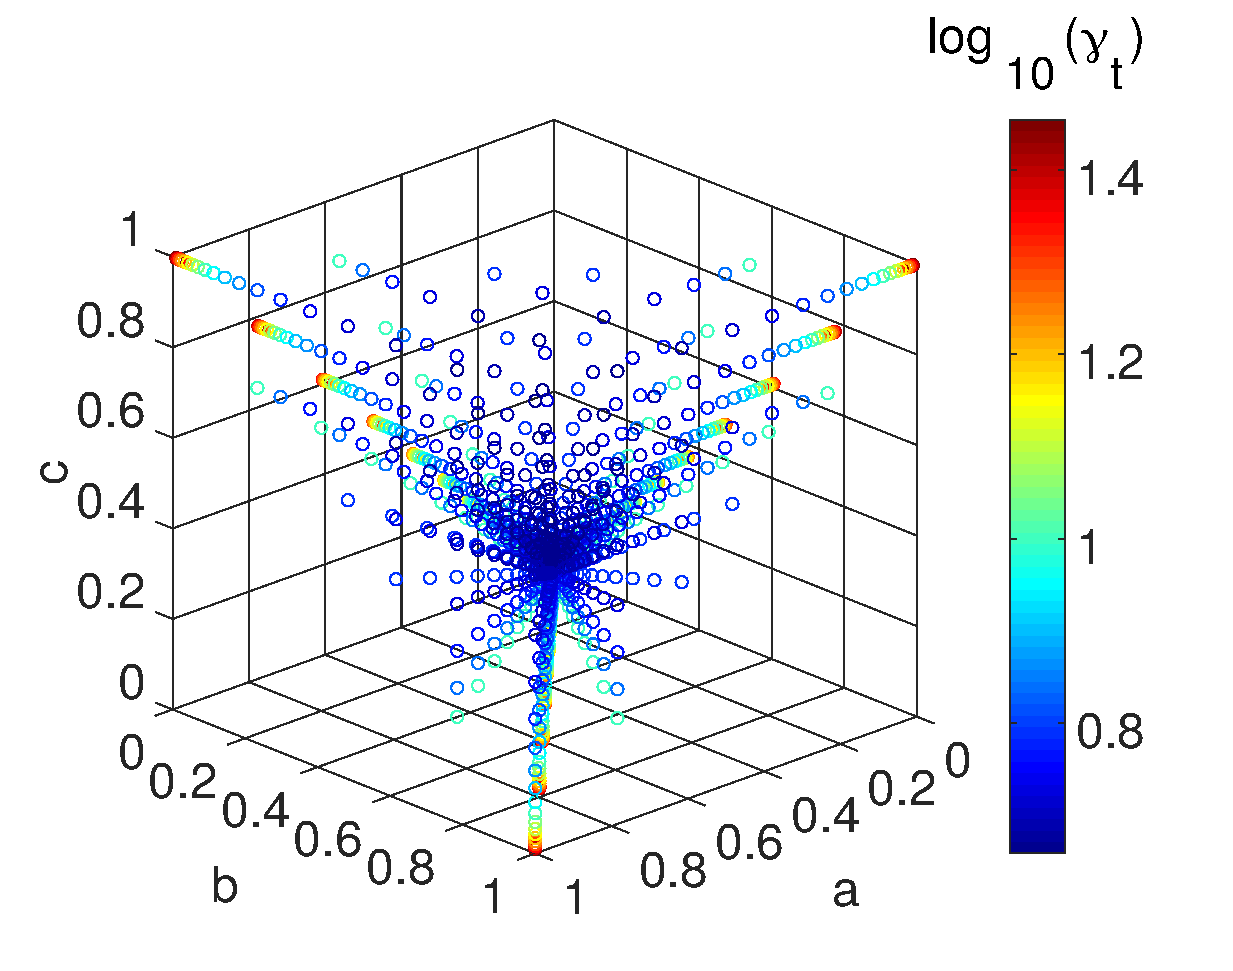
\includegraphics[width=0.45\textwidth]{section1-gammat.eps}
\caption{Solid generated by some possible values of $log_{10}(\gamma_t(a,b,c))$.}
\label{fig:section1-gammat}
\end{figure}

To obtain the minimum value $\gamma_t(a,b,c)$ in this solid we need 
calculate $\frac{\partial \gamma_t(a,b,c)}{\partial a}=0$,
$\frac{\partial \gamma_t(a,b,c)}{\partial b}=0$
and $\frac{\partial \gamma_t(a,b,c)}{\partial c}=0$;
but by the symmetry of three equations, 
and the experience in the calculus made in the Section \ref{subsec:gammar},
we know that the minimum can be reach when $a=b=c$;
this mean when $\gamma_t(a,a,a)=\frac{6}{\sqrt[4]{3}}\approx 4.5590$; so that
\begin{equation}
4.5590 \leq \gamma_t(a,b,c) 
\end{equation}

%%%%%%%%%%%%%%%%%%%%%%%%%%%%%%%%%%%%%%%%%%%%%%%%%%%%%%%%%%%%%%%%%%%%%%%%%%%%%%%%
\subsection{Digest of $\gamma$ values}
The $\gamma$ values obtained in the last sequences can be order as show the
Fig. \ref{fig:section1-diagrama1}.
\begin{figure}[h!]
\centering
\includegraphics[width=0.45\textwidth]{section1-diagrama1.eps}
\caption{$\gamma$ values of some geometric figures.}
\label{fig:section1-diagrama1}
\end{figure}
In this figure we can observe that if only we use the value $\gamma$,
 exist a point when an ellipse is indistinguishable of a rectangle,
and this happen when $\gamma_e(a,b)=4$, and consequently
\begin{equation}
4=\frac{4\int \limits_{0}^{\frac{\pi}{2}}{\sqrt{a^2-(a^2-b^2)sin^2(\theta)}d\theta}}{\sqrt{\pi ab}},
\end{equation}
\begin{comment}
\begin{equation}
\sqrt{\pi ab}=\int \limits_{0}^{\frac{\pi}{2}}{\sqrt{a^2-(a^2-b^2)sin^2(\theta)}d\theta},
\end{equation}
\begin{equation}
\sqrt{\pi ab}=\int \limits_{0}^{\frac{\pi}{2}}{a\sqrt{1-\left(1-\left(\frac{b}{a}\right)^2\right)sin^2(\theta)}d\theta},
\end{equation}
\begin{equation}
\sqrt{\pi} \sqrt{\frac{b}{a}}=\int \limits_{0}^{\frac{\pi}{2}}{\sqrt{1-\left(1-\left(\frac{b}{a}\right)^2\right)sin^2(\theta)}d\theta},
\end{equation}
\begin{equation}
\sqrt{\pi} \sqrt{r}=\int \limits_{0}^{\frac{\pi}{2}}{\sqrt{1-\left(1-r^2\right)sin^2(\theta)}d\theta},
\end{equation}
\end{comment}
\begin{equation}
r=\frac{\left(\int \limits_{0}^{\frac{\pi}{2}}{\sqrt{1-\left(1-r^2\right)sin^2(\theta)}d\theta}\right)^2}{\pi},
\end{equation}
being $r=\frac{b}{a}$. Where $r$ can be found using iteratively the equation
\begin{equation}
r_k=\frac{\left(\int \limits_{0}^{\frac{\pi}{2}}{\sqrt{1-\left(1-{r_{k-1}}^2\right)sin^2(\theta)}d\theta}\right)^2}{\pi},
\end{equation}
from $r_0=1$ until that $r_k\approx r_{k-1}$, where we declare that $r=r_k$.
Thus, we obtain with this method that 
a ellipse with $\gamma_e(a,b)=4$ have values $a$ and $b$ that fulfill the ratio $\frac{b}{a}\approx 0.437891897721079$.
With all these considerations we can show in the
Fig. \ref{fig:section1-gammae-square} a ellipse and a square with the same area and a $\gamma=4$.
\begin{figure}[h!]
\centering
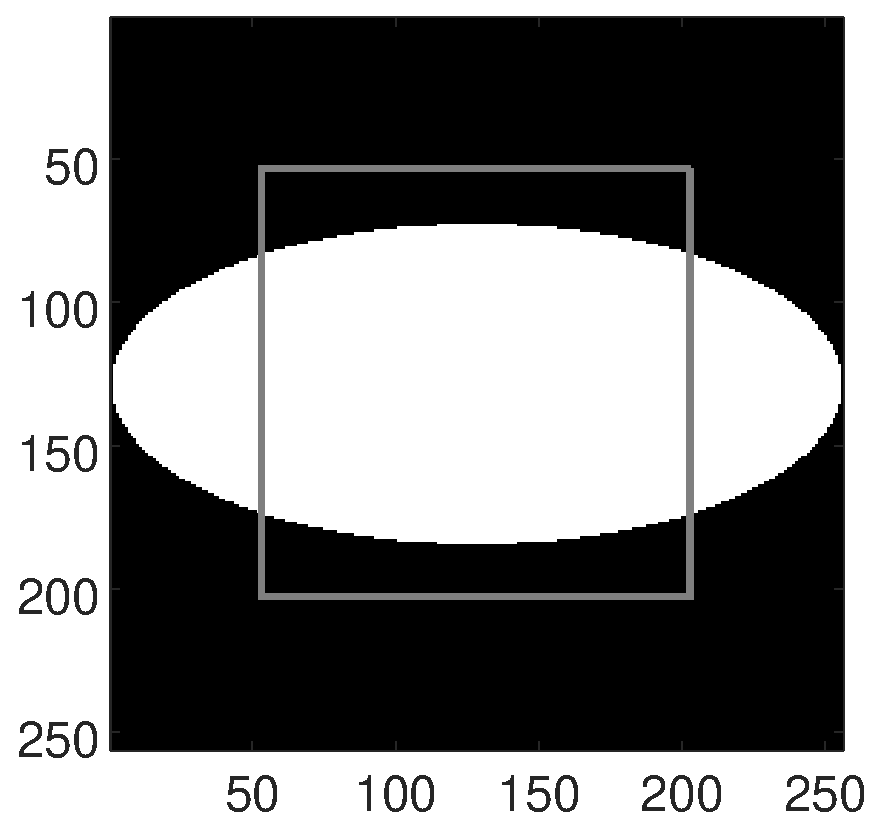
\includegraphics[width=0.3\textwidth]{section1-gammae-square.eps}
\caption{Ellipse and square with the same area and a $\gamma=4$.}
\label{fig:section1-gammae-square}
\end{figure} 
